\documentclass[12pt]{article}
\pagestyle{empty}

\usepackage[top=2cm,left=1cm,right=1cm,bottom=2cm]{geometry}
\usepackage[all]{xy}
\usepackage[fleqn]{amsmath}
\usepackage{subcaption}
\usepackage{graphicx}
\usepackage{textcomp}
\usepackage[none]{hyphenat}
\begin{document}


\begin{center}
\Large{Currency Converter}

\large{Spring 2018}
\end{center}
\vspace{3 mm}
Michael Ibanez
\vspace{5 mm}

\begin{enumerate}

%%%%%%%%%%%%%%%%%%%%%%%%%%%%%%%%%%%%%%%%%%%
\item   Outline : 

\subitem 
	This project is a currency converter that use CurrenyLayer's API to get real time conversions from one currency to another.


%%%%%%%%%%%%%%%%%%%%%%%%%%%%%%%%%%%%%%%%%%%
\item   Vision Statement : 
	
\subitem
	To create an application with a Graphical User Interface that will demonstrate proper use of Java tools and documentation


%%%%%%%%%%%%%%%%%%%%%%%%%%%%%%%%%%%%%%%%%%%
\item   All roles

\begin{enumerate}
	\item Client
	\item MainWindow
	\item MenuController
	\item LoadingController
	\item SettingsController
	\item ConvertController
	\item ExitMain
\end{enumerate}


%%%%%%%%%%%%%%%%%%%%%%%%%%%%%%%%%%%%%%%%%%%
\item   Gant diagram with timing: 

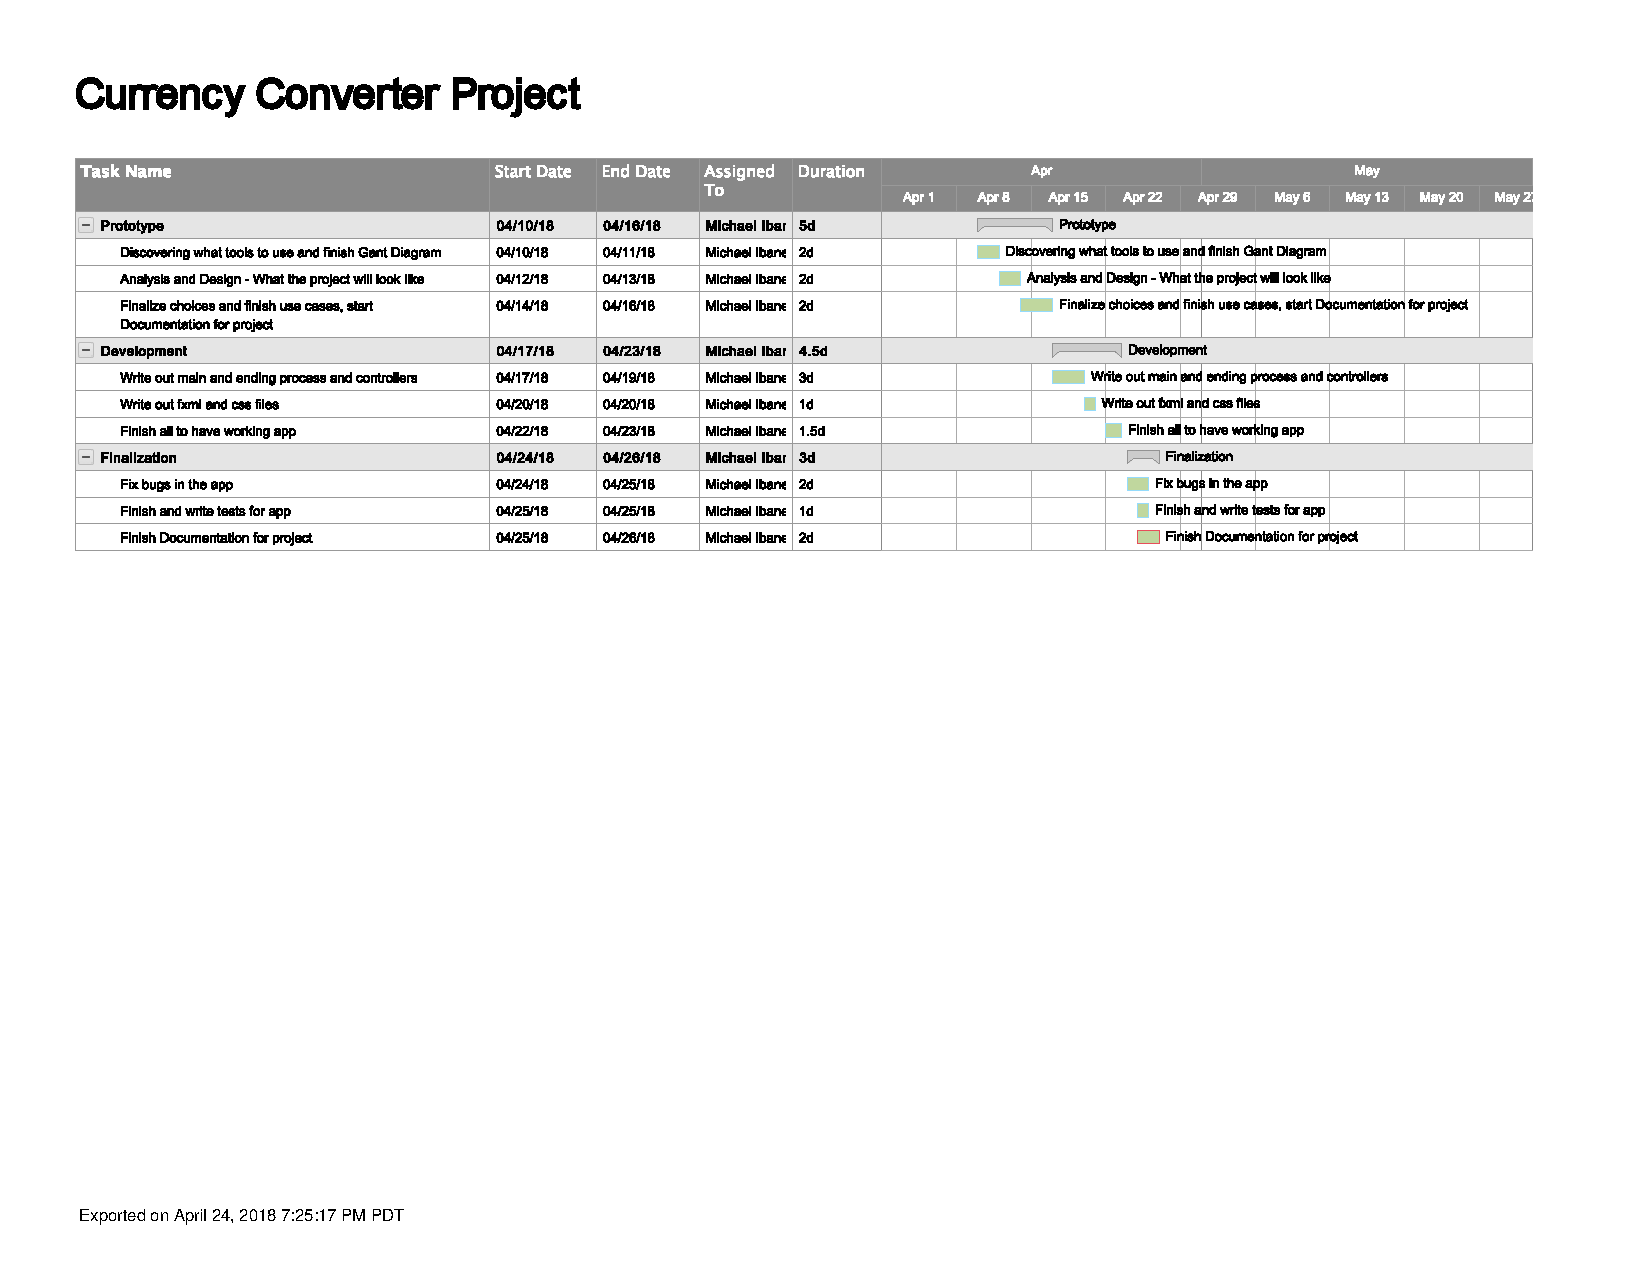
\includegraphics[scale=0.5]{GantDiagram.pdf}


%%%%%%%%%%%%%%%%%%%%%%%%%%%%%%%%%%%%%%%%%%%
\item   Requirements : 

\subitem Injection option given to user to inject css into files
\subitem Easy to navigate
\subitem User interface is simple to use
\subitem Should comply with business rules
\subitem Software is developed with five or more design patterns
\subitem User interface should be consistent with color, font, and size.
\subitem Software should be able to convert one currency to another
\subitem Software should convert in a quick amount of time(2 seconds > )



%%%%%%%%%%%%%%%%%%%%%%%%%%%%%%%%%%%%%%%%%%%
\item   Business rules (3 or more) : 

\subitem Software is developed with 1000 LOC at least
\subitem Software should be tested with JUnit
\subitem Software should be mainted with Git and at least 30 commits
\subitem Software needs to have a graphical user interface
\subitem Software should be able to convert from any currency to any other currency
\subitem Software should only convert currencies from the CurrencyLayer API


%%%%%%%%%%%%%%%%%%%%%%%%%%%%%%%%%%%%%%%%%%%
\item   Use cases (3 or more) : 

Use Case Name: Currency Convert

Actors: MenuScreenController , Client , ConvertScreenController

Triggers : The Client has past loading screen and wants to convert currencies

Preconditions : Client has passed loading screen.

Post-conditions : Client will know the currency conversion of a single unit, and the amount the Client entered. System will be ready for another currency as soon as it is over.

Normal Flow:

\begin{enumerate}
	\item Client will indicate that he/she will want to convert currencies
	\item MainWindow will load the menu screen 
	\item The client will then choose their option to go the convert screen
	\item MenuScreenController will then load the convert screen
	\item Client will input amount of currency to change
	\item Client will choose the currencies to convert from
	\item ConvertScreenController will send the call to CurrencyLayer API
	\item ConvertScreenController send the information back to Client by updating window fields
	\item Client will see results
\end{enumerate}

Alternate flows

bA1 : MainWindow will not load
\newline bA2 System will display error message and wait for Client to close application

eA1 : Client input invalid numers
\newline eA2 System will display error message and wait for Client to choose valid numers

Summary : The Client, after going past loadingScreenController, will head to the menu(MenuScreenController) and then the Client will choose the convert button to go to the convert page (ConvertScreenController) from there the user inputs in the value to convert as well as the two currencies to convert from.



\subitem --------------
\newline Use Case Name: InjectCSS

Actors: MenuScreenController , Client , SettingScreenController, System

Triggers : The Client intents to go to the settings and inject into a css file

Preconditions : The Client has opened application.

Post-conditions : Client will have injected his choice of elements into a css file and will then be able to reload project to see updated settings

Normal Flow:

\begin{enumerate}
	\item Client will indicate that he/she will want to inject into css files
	\item MainWindow will load the load screen
	\item The client will then choose their option to go the menu scree
	\item LoadingScreenController will then load the menu screen
	\item Client will then choose to go the settings screen
	\item MenuScreenController will then load the settings screen
	\item Client will input class, property, and value of property to inject 
	\item Client will inject 
	\item ConvertScreenController will then inject into the css files the chosen values
	\item System will have the files changed
	\item Client will reload application to see results
\end{enumerate}

Alternate flows

bA1 : MainWindow will not load
\newline bA2 System will display error message and wait for Client to close application

cA1 : Client chose wrong option
\newline cA2 System will display othermenu that has a back button
\newline cA3 Client will go back and choose correct option

gA1 : Client left fields blank or incorrect values
\newline gA2 ConvertSystemController will pick default values to load the incorrect or blank values

Summary : The Client, after loading application, will head to the loading screen(loadingScreenController) and then the Client will choose the menu button to go to the menu page (MenuScreenController) then the Client will choose the settings button to go to the settings page (SettingsScreenController). The client will then choose appropriate calues for the injector and after hitting the inject button, will reload the application to see updated files.



\subitem -----------------
\newline Use Case Name: Exit Converter

Actors: System, Client, MainWindow, ExitMain

Triggers : The Client wants to close application

Preconditions : Client has loaded appplication

Post-conditions : Client have shutdown the application

Normal Flow:

\begin{enumerate}
	\item Client will indicate that he/she will want to exit application
	\item MainWindow will load the current screen it is at
	\item The client will then choose their option to exit the application by exit , or X button
	\item MainWindow will ask user if they really want to quit application
	\item Client will choose option to close
	\item MainWindow invokes its option to close window
	\item System will close the application
\end{enumerate}

Alternate flows

bA1 : MainWindow will not load
\newline bA2 System will display error message and wait for Client to close application

eA1 : Client ichoose option to not close application
\newline eA2 System will display its prior screen and continue on

Summary : The Client, after loading application, will choose the option to close the application by either an exit or X button which will then ask the user if she/he really wants to quit application. The system will then close the application after the Client chooses to do so.



%%%%%%%%%%%%%%%%%%%%%%%%%%%%%%%%%%%%%%%%%%%
\item   Use Case diagram for all roles : 
\newpage
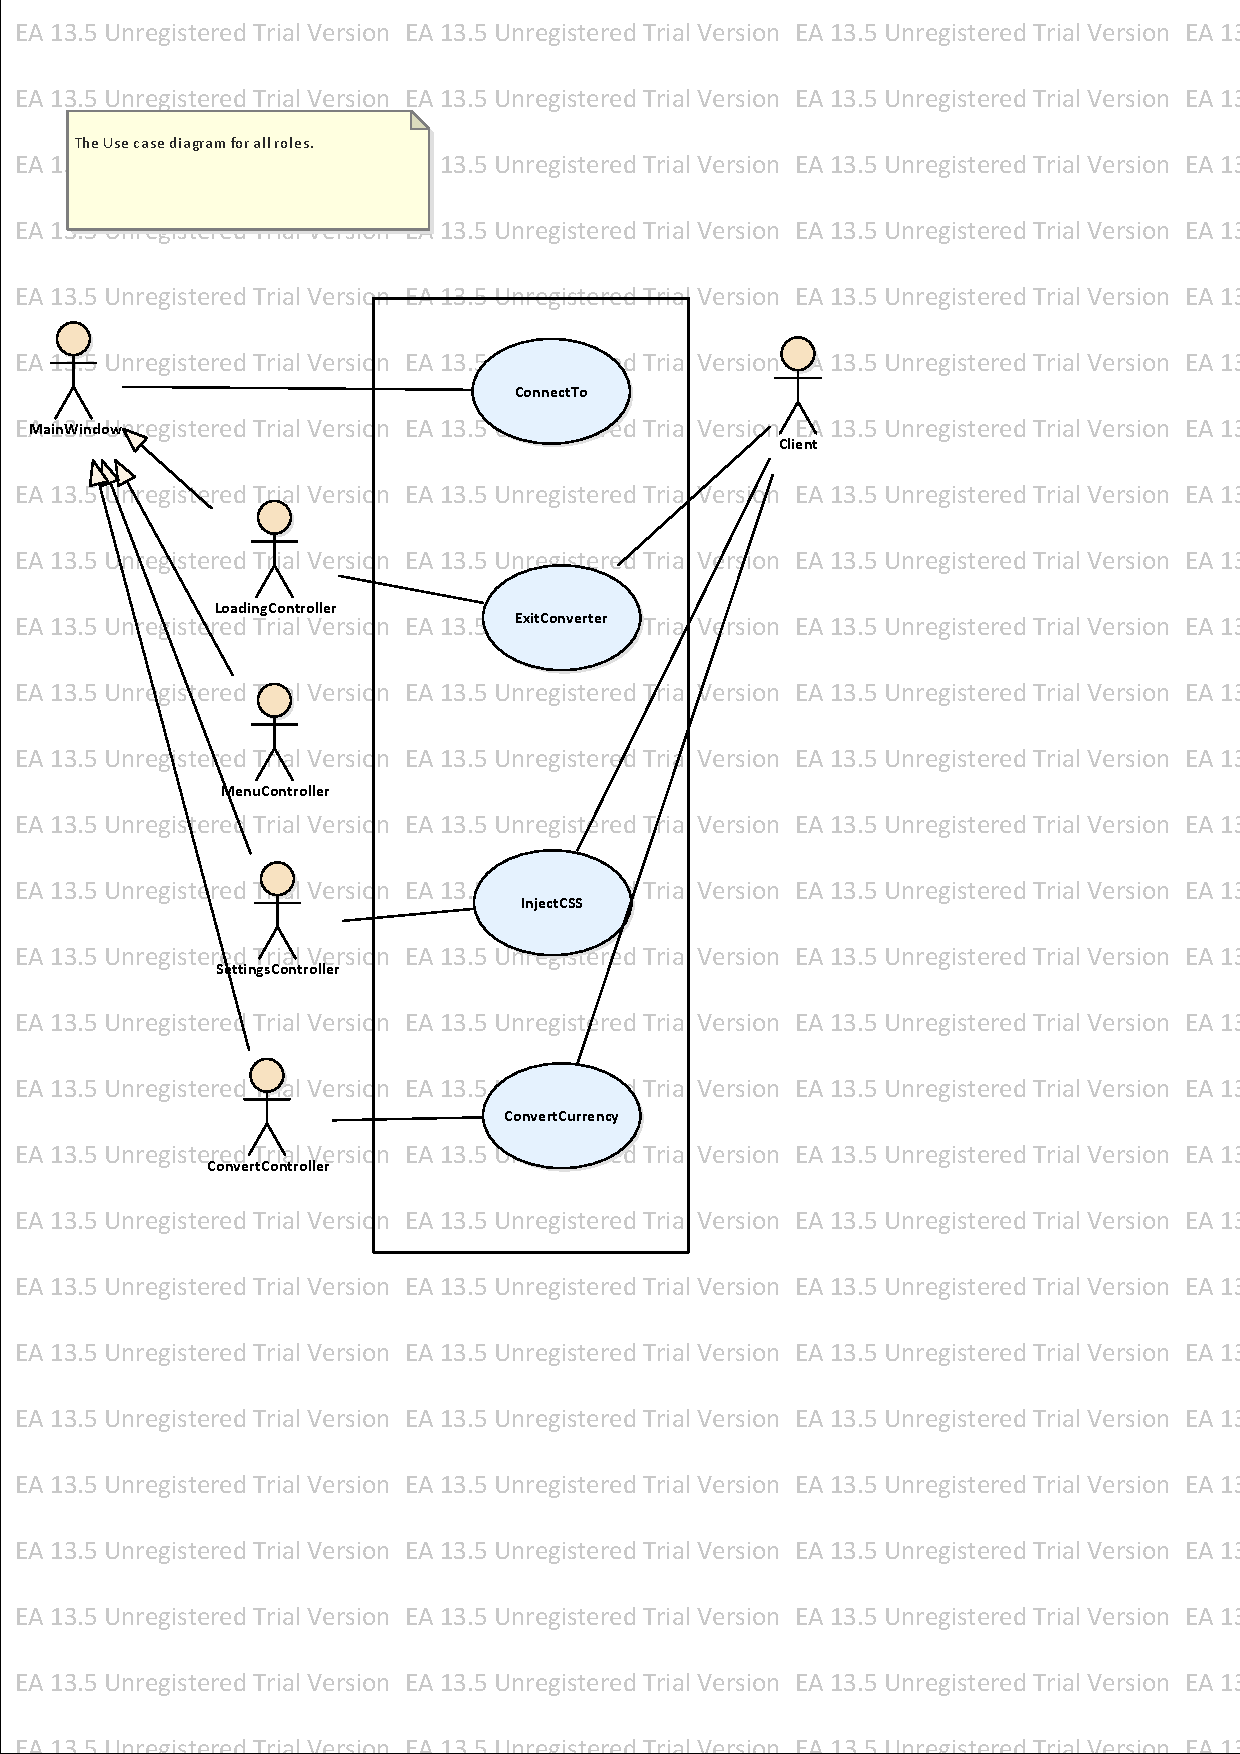
\includegraphics[scale=0.8]{useCase.pdf}
\newpage

%%%%%%%%%%%%%%%%%%%%%%%%%%%%%%%%%%%%%%%%%%%
\item   System Operations : 

\subitem main(String[] args)
\subitem start(Stage)
\subitem connectToLoading()
\subitem connectToMenu()
\subitem connectToSettings()
\subitem connectToConvert()
\subitem closeProgram(Stage)
\subitem Initialize(URL,Resourcebundle)
\subitem getCurr()
\subitem getWindow()
\subitem setWindow()
\subitem check()
\subitem yesAction(ActionEvent)
\subitem noAction(ActionEvent)
\subitem linkedInAction(ActionEvent)
\subitem githubAction(ActionEvent)
\subitem back(ActionEvent)
\subitem write(File)
\subitem convertAction(ActionEvent)
\subitem settingAction(ActionEvent)
\subitem creditsAction(ActionEvent)
\subitem creditsActionFile()
\subitem sendLiveRequest()



%%%%%%%%%%%%%%%%%%%%%%%%%%%%%%%%%%%%%%%%%%%
\item   Domain model : 

\newpage
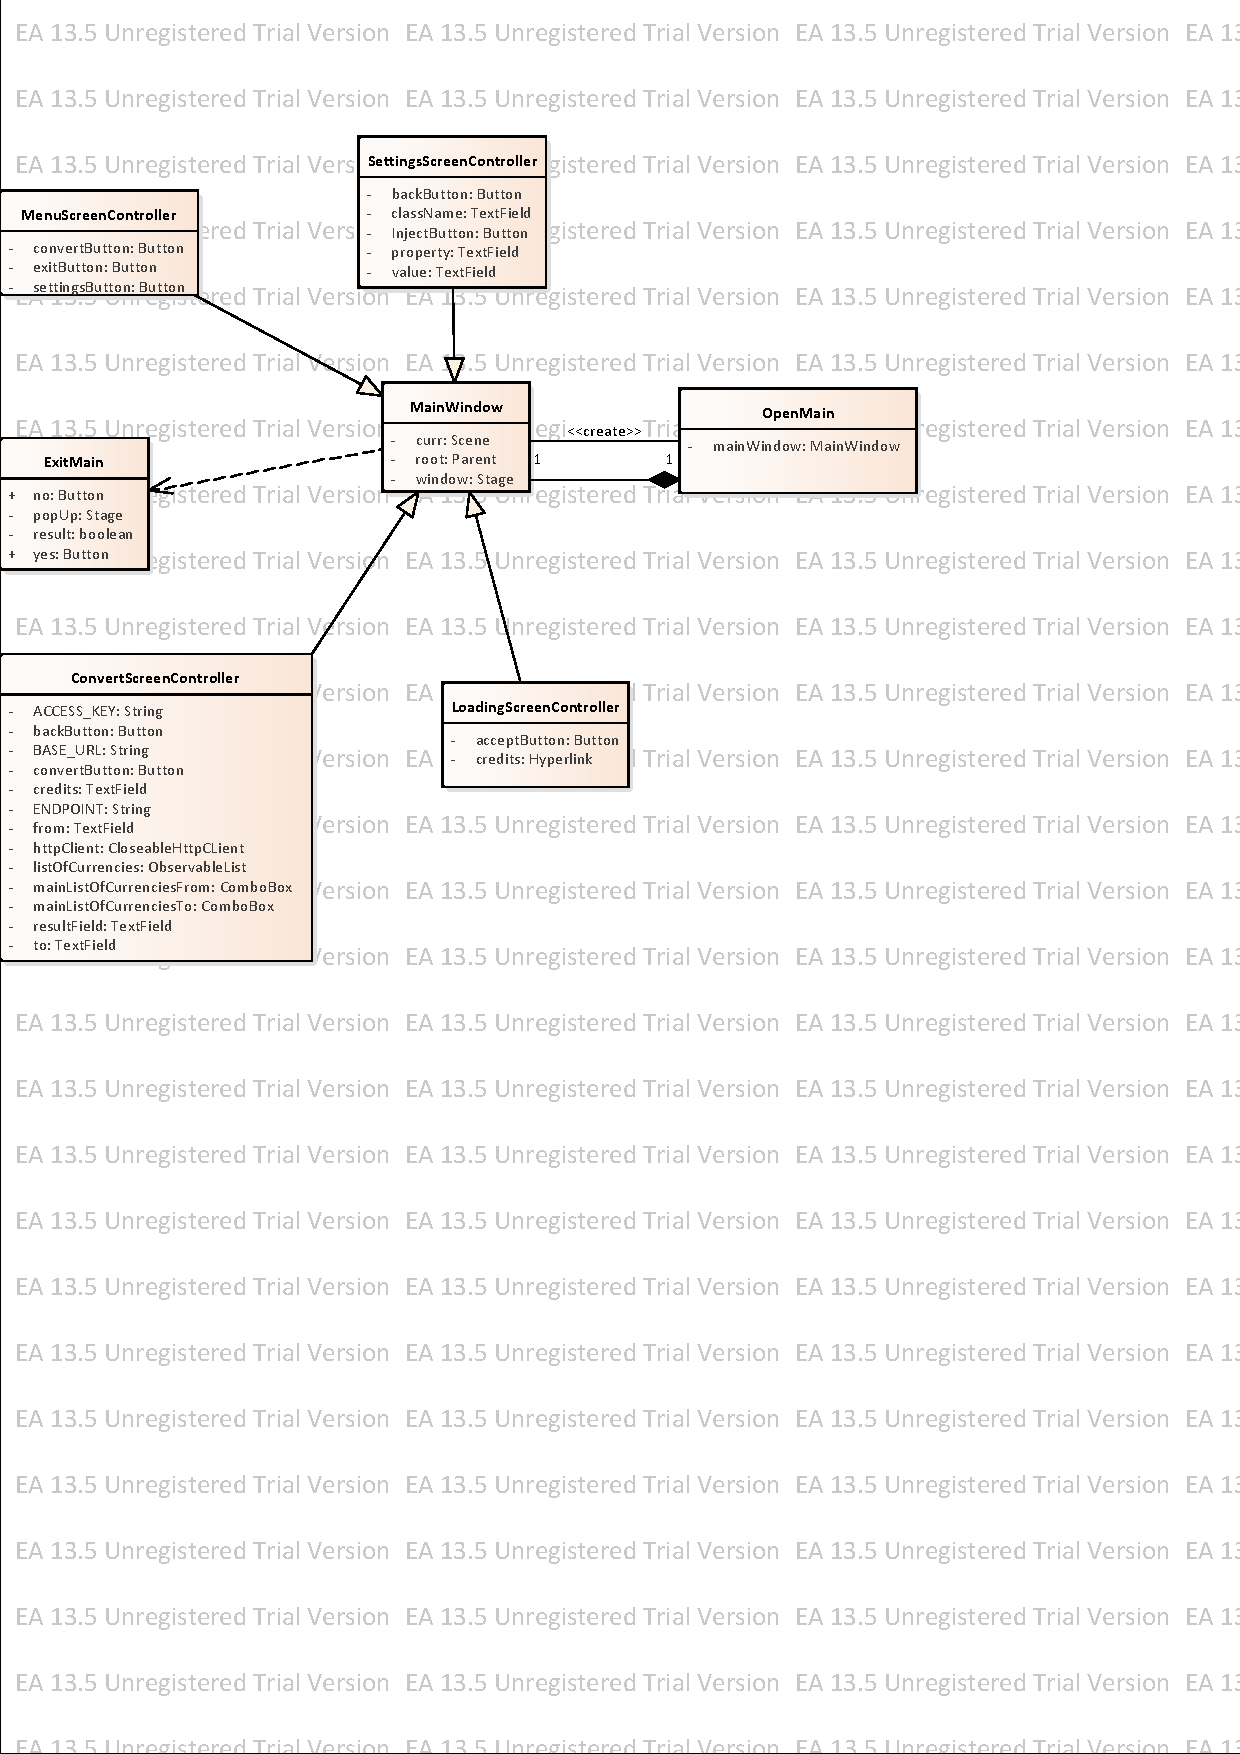
\includegraphics[scale=0.8]{domainModel.pdf}
\newpage


%%%%%%%%%%%%%%%%%%%%%%%%%%%%%%%%%%%%%%%%%%%
\item   Operation contracts: 

\begin{enumerate}
\item Contract CO2: convertAction
\newline Operation:convertAction(ActionEvent e)
\newline Cross References - Use Cases: Currency Convert
\newline Pre-conditions: Client has loaded application
\newline Post-conditions: Client now knows a new currency conversion
\newline ConvertScreenController has made a call to the CurrencyLayerAPI
\newline ConvertScreenController is ready to make another conversion
\newline
\item Contract CO2: creditsAction
\newline Operation: creditsAction(ActionEvent e)
\newline Cross References - Use Cases:
\newline Pre-conditions: Client has loaded application into menu/ setting/ convert screen
\newline Post-conditions: Client will see a credit to the author in console
\newline
\item Contract CO2: back/exit
\newline Operation: back(ActionEvent e)
\newline Cross References - Use Cases: exitConverter
\newline Pre-conditions: Client has loaded application
\newline Post-conditions: Client has exited and properly closed application
\newline
\item Contract CO2: connectToMenu
\newline Operation: connectToMenu()
\newline Cross References - Use Cases: 
\newline Pre-conditions: Client has loaded application
\newline Post-conditions: Client is now in the Menu Screen
\newline
\item Contract CO2: connectToSetting
\newline Operation: connectToSetting()
\newline Cross References - Use Cases: 
\newline Pre-conditions: Client has loaded application and is in the menu screen
\newline Post-conditions: Client is now in the Setting screen
\newline
\item Contract CO2: connectToConvert
\newline Operation: connectToConvert()
\newline Cross References - Use Cases: 
\newline Pre-conditions: Client has loaded application and is in the menu screen
\newline Post-conditions: Client is now in the Convert screen
\newline
\item Contract CO2: injectAction
\newline Operation: injectAction(ActionEvent e)
\newline Cross References - Use Cases: InjectCSS
\newline Pre-conditions: Client has loaded application and is in the settings menu
\newline Post-conditions: Client has now loaded a customized version of css files
\newline Client can reload application to see new effects
\newline
\item Contract CO2: initialize
\newline Operation: initialize(URL l, ResourceBundle r) 
\newline Cross References - Use Cases: 
\newline Pre-conditions: Client has started application
\newline Post-conditions: Client has now loaded the proper css and fxml files
\newline Client can see the effects of the files
\end{enumerate}


%%%%%%%%%%%%%%%%%%%%%%%%%%%%%%%%%%%%%%%%%%%
\item   Design model : 

\newpage
\includegraphics[scale=0.8]{dESIGNModel.pdf}
\newpage


%%%%%%%%%%%%%%%%%%%%%%%%%%%%%%%%%%%%%%%%%%%
\item   Justification of GRASPS : 

\subitem Creator : Was MainWindow and Initializable that the ScreenControllers were inherited from, this seemed appropriate in order to have an order of classes
\subitem Information expert : Only classes that needed to know its specific details had access to it, like convertAction in ConvertScreenController was only available to that class. Each class was made specifically for dealing with specific parts, like exitMain was always used for exiting the application, SettingScreenController was always used for injection to the css files
\subitem Low Coupling : Coupling was great here since the classes that depended on something else were the Controller and MainWindow classes. If something changed in MainWindow, it wasn't difficult to change it in the other classes since it was an extension of it. MainWindow was extended by the Controller classes, but that was pretty much all it had so the coupling was still good
\subitem Controller : This looked justified by how each Controller, ExitMain, and MainWindow each took user response when needed to, so the user wasn't always going through the same object
\subitem High Cohesion : Cohesion was more towards the middle since the Controllers classes only delegated its own functions. 
\subitem Law of demeter : Other classes weren't allow to access or know about the other classes functions except for the Controllers to MainWindow
\subitem Polymorphism : Justified by having each Controller implementing Initializable and then overriding the initializable function each time to a certain implementation
\subitem Pure Fabrication : I made a class specifically to handle the exit methods(ExitMain) which was made up in order to support high cohesion, low coupling, and reuse of the code.




%%%%%%%%%%%%%%%%%%%%%%%%%%%%%%%%%%%%%%%%%%%
\item   Sequence diagrams (for 3 use cases) : 

\subitem 1 : ConvertCurrency
\newpage
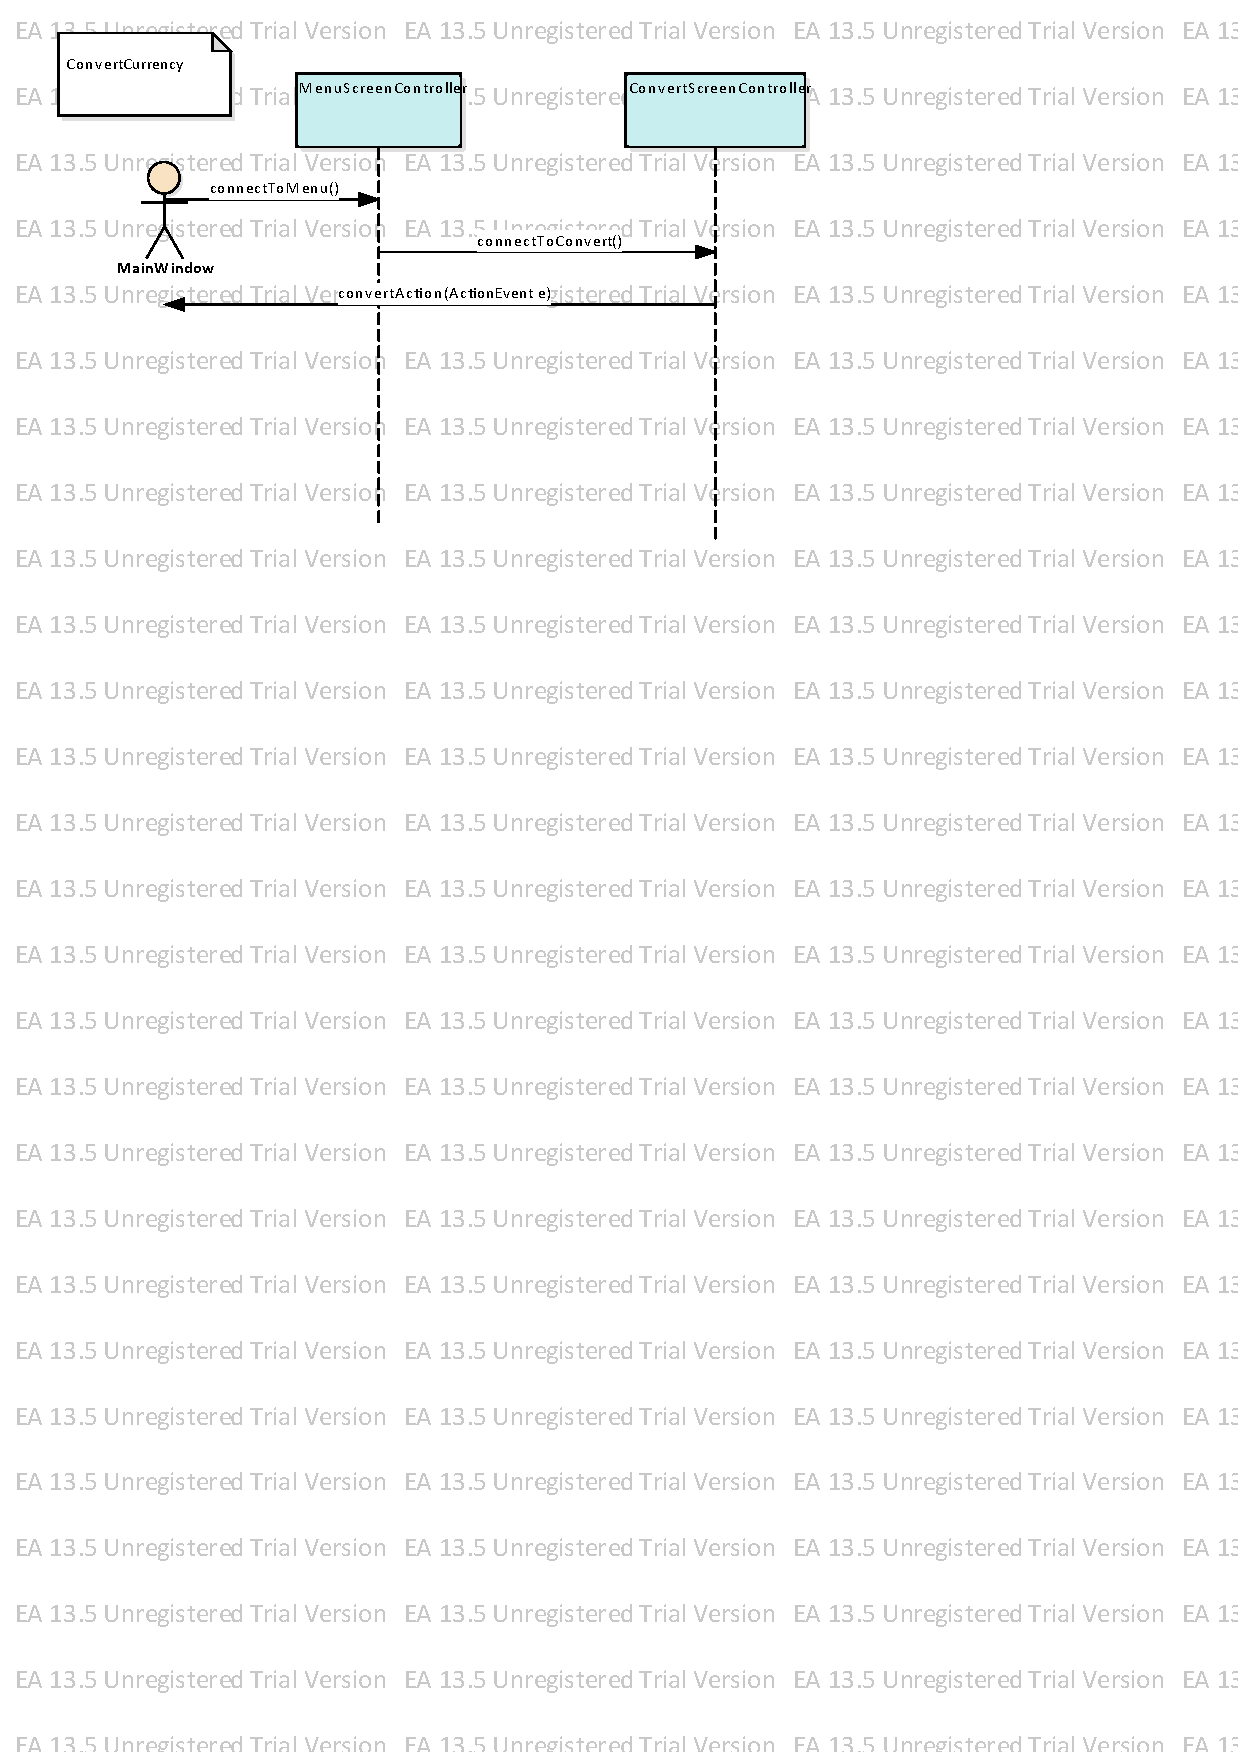
\includegraphics[scale=0.8]{convertCurrency.pdf}
\newpage

\subitem 2 : InjectCSS
\newpage
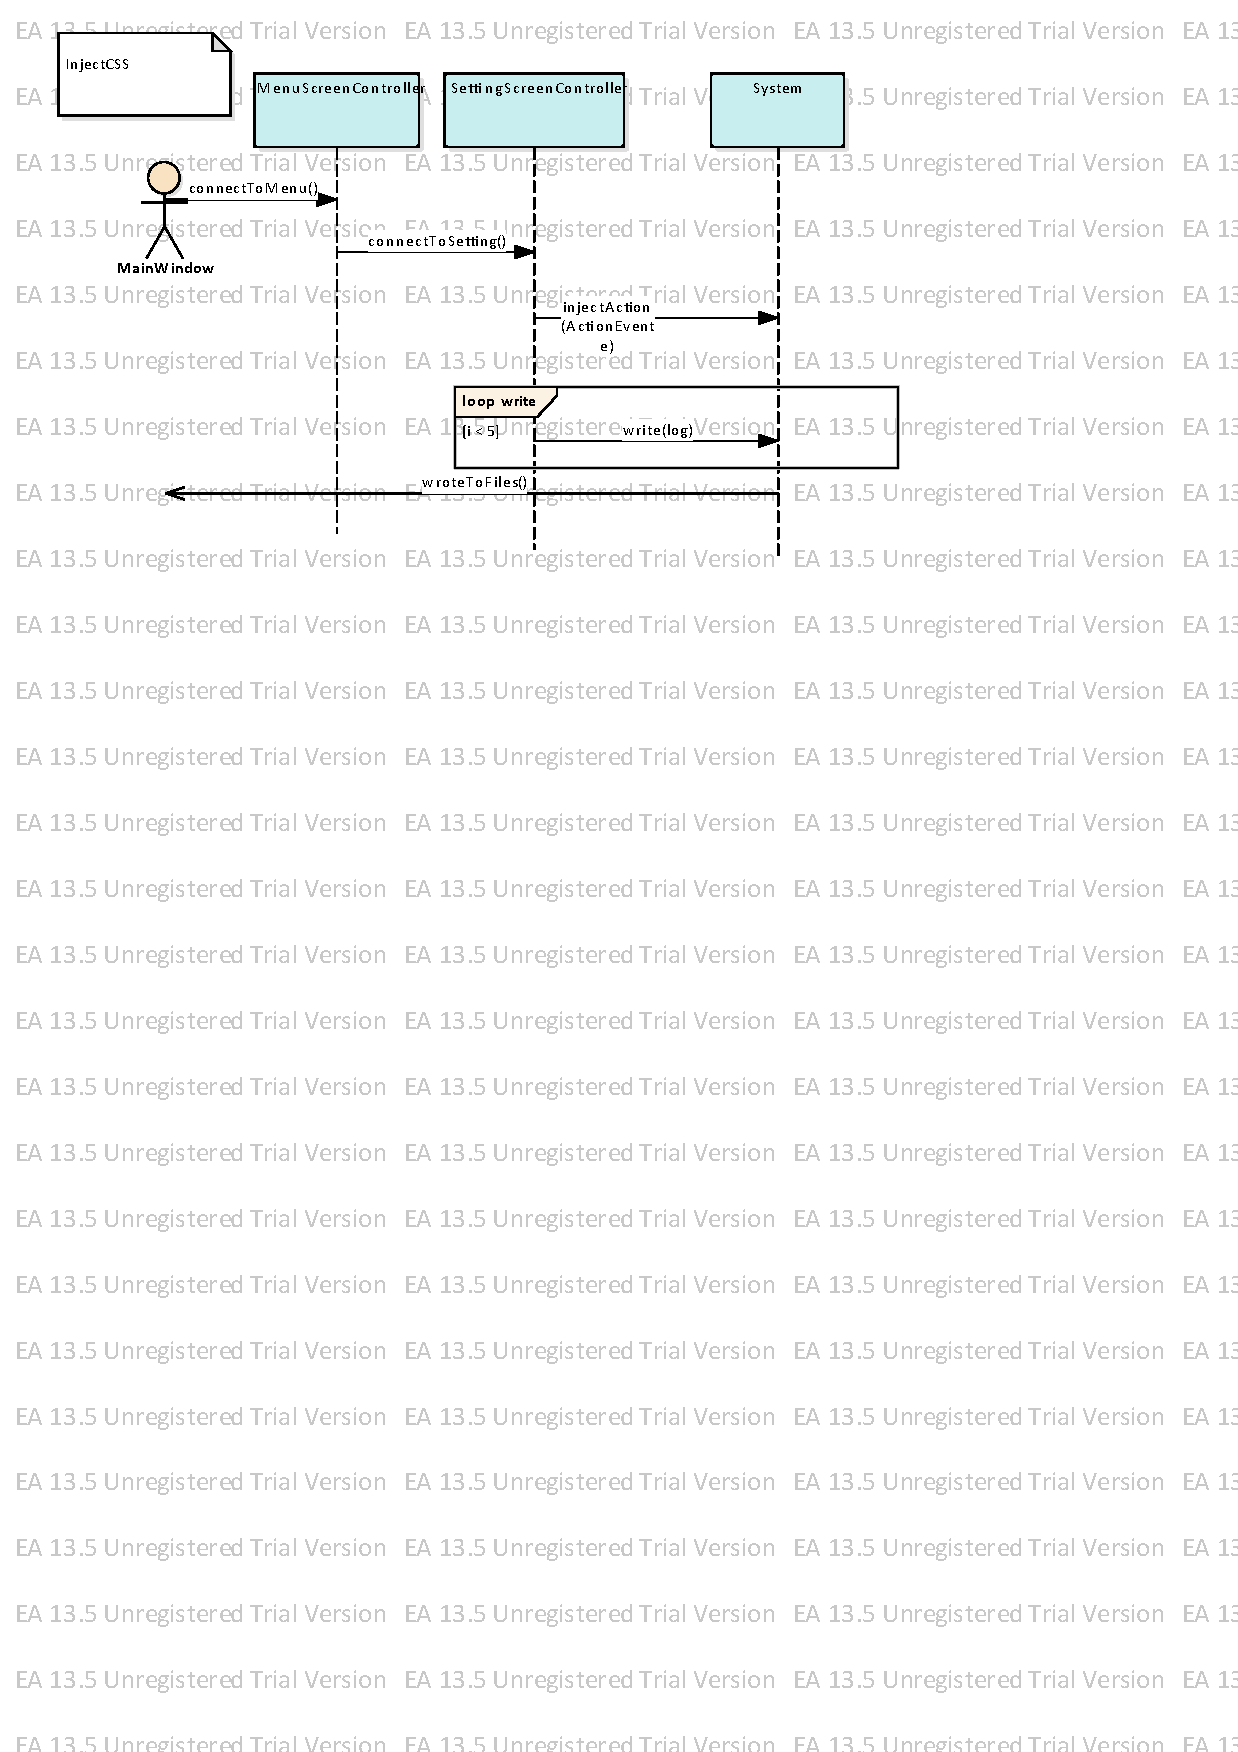
\includegraphics[scale=0.8]{injectAction.pdf}
\newpage

\subitem 3 : exitConverter
\newpage
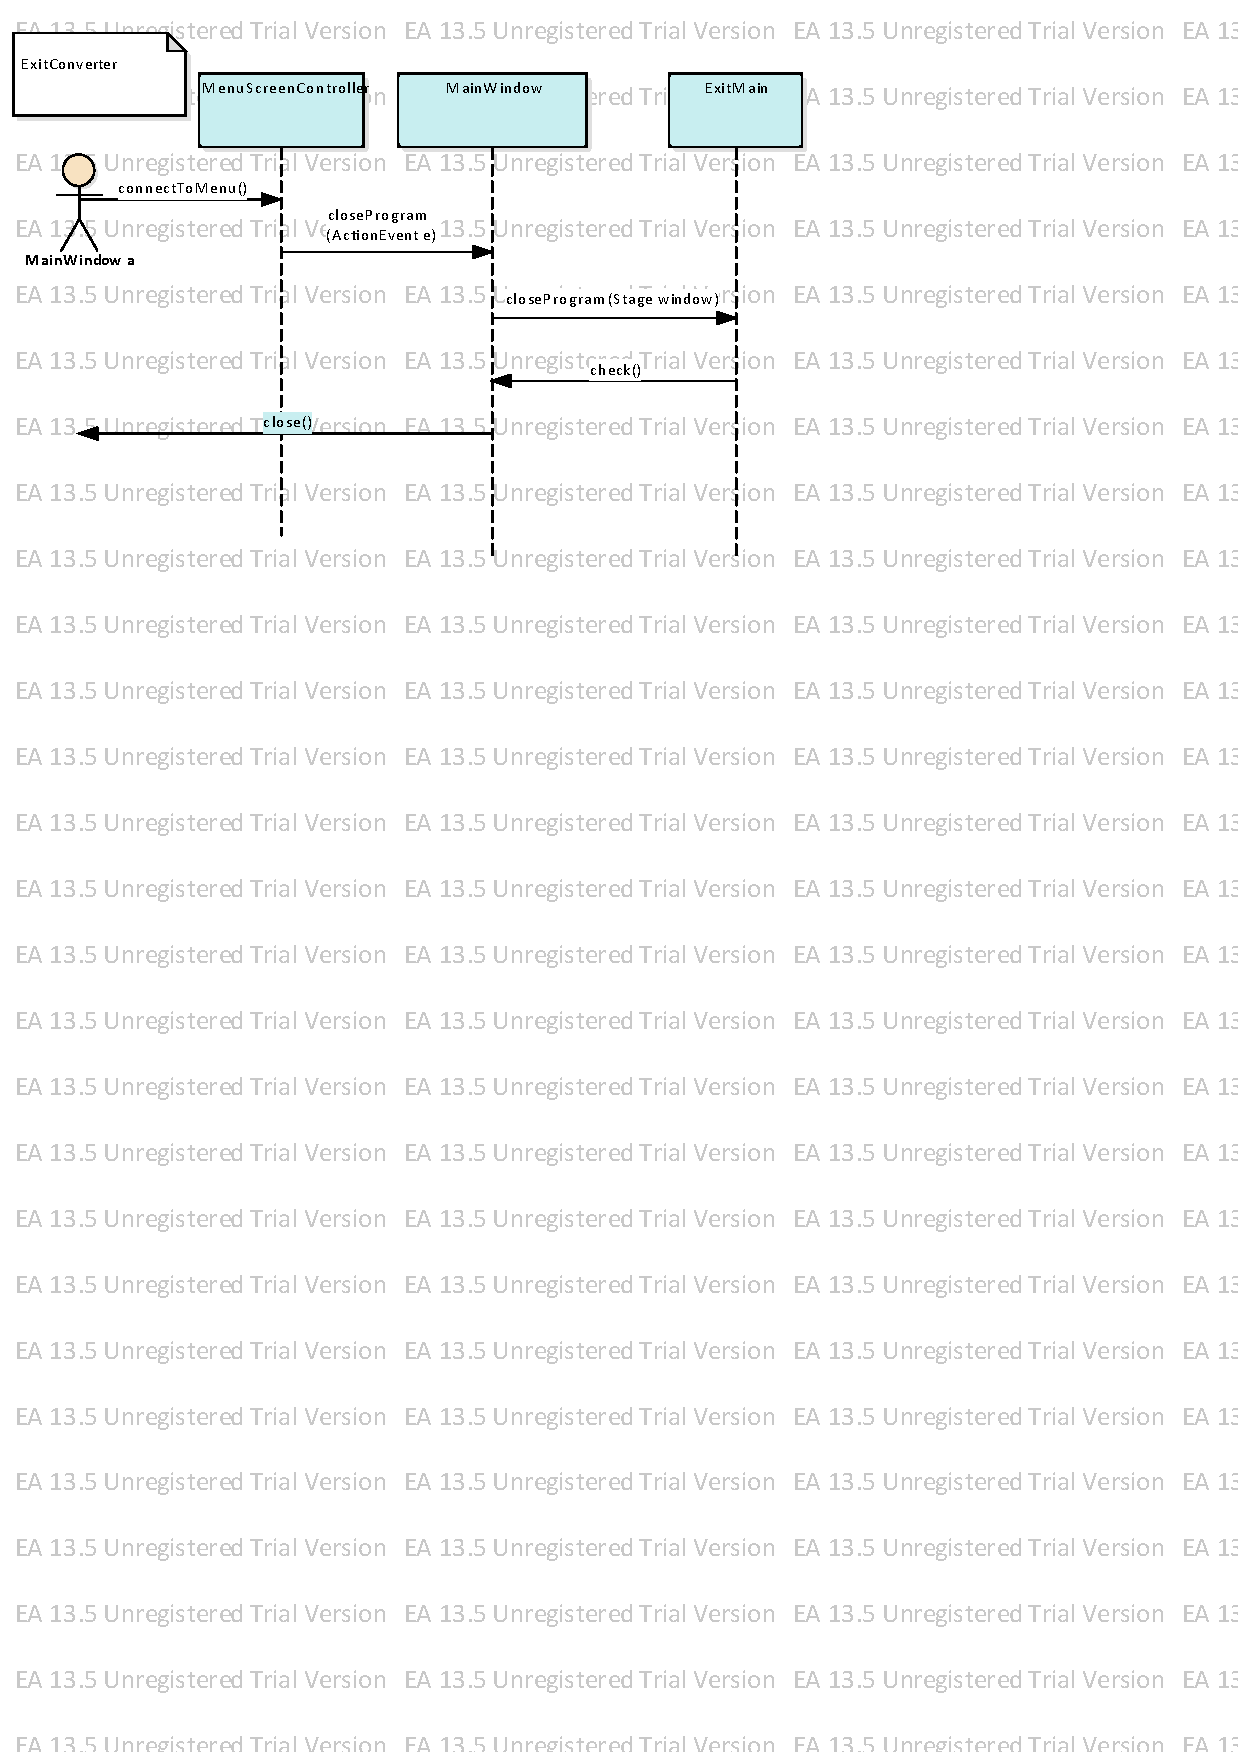
\includegraphics[scale=0.8]{exitConverter.pdf}
\newpage


%%%%%%%%%%%%%%%%%%%%%%%%%%%%%%%%%%%%%%%%%%%
\item  Where did you use a design pattern and why?
	\begin{enumerate}
			\item Command
			\subitem This was used in a lot of the buttons like creditAction, creditActionToFile, convertAction, etc. Here when a button was pressed, the appropriate function was called which then called other functions.
	\end{enumerate}

	\begin{enumerate}
		\item Decorator
		\subitem This was used in the initlization of each ScreenController  since each one would like to have different settings. I used it here because it was helpful to change what each ScreenController initiliazed to instead ofinitiliazing everything.
	\end{enumerate}
	
	\begin{enumerate}
		\item Facade
		\subitem This was used in hiding the implemetation of each MainWindow by having the user run the program from a OpenMain instance. This seemed best here so the user couldnt see anything past the OpenMain instance.
	\end{enumerate}

	\begin{enumerate}
		\item Mediator
		\subitem This was used in the ScreenControllers especially for convertScreenController because it separates MainWindow from the action of converting currency (which has an API call to CurrencyLayer).
	\end{enumerate}
	
	\begin{enumerate}
		\item Proxy
		\subitem This was used in closeProgram because it was useful to be able to have a single function that all the ScreenControllers can use to exit the application at any time. The proxy was the window that popped up and ask the user if he/she really wanted to quit the application, and if so would return to tell the user.
	\end{enumerate}

%%%%%%%%%%%%%%%%%%%%%%%%%%%%%%%%%%%%%%%%%%%
\item   LOC : 2173

%%%%%%%%%%%%%%%%%%%%%%%%%%%%%%%%%%%%%%%%%%%
\item   Sources used : 

	\begin{enumerate}
	\item https://www.programcreek.com/java-api-examples/?class=javafx.stage.Stage\&method=setOnCloseRequest
	\item https://examples.javacodegeeks.com/desktop-java/javafx/fxml/javafx-fxml-controller-example/

	\end{enumerate}

\end{enumerate}
\newpage
\end{document}






